\documentclass[handout]{beamer}

\usepackage{fontspec} 
% \usepackage{lsp-makros}
\useoutertheme{lsp}

\usepackage{lsptitle}

\def\two@digits#1{\ifnum#1<10 0\fi\number#1}
\def\mytoday{\two@digits{\number\day}.\two@digits{\number\month}.\number\year}


\usepackage{xspace,multicol}
\newcommand{\latex}{\LaTeX\xspace}
\usepackage{tikz}


\newcounter{lastpagemainpart}
\footnotesep0pt
\renewcommand{\footnoterule}{}
\usefootnotetemplate{
  \noindent
  \insertfootnotemark\insertfootnotetext}

\let\beamerfn=\footnote
\renewcommand{\footnote}[1]{%
\let\oldfnsize=\footnotesize%
\let\footnotesize=\tiny%
\beamerfn<\thebeamerpauses->{#1}%
\let\footnotesize=\oldfnsize}


\date{2018-01-10}

\usepackage{eurosym}  
 
\renewcommand{\centerline}[1]{\hfill#1\hfill\hfill\mbox{}}


\title{Language Science Press}
% \institute{FU Berlin}
\author[LangSci]{Sebastian Nordhoff 
% \mbox{\tiny\url{https://github.com/langsci/lsp-presentations/blob/master/oat2017books/presentation.pdf}}
}



\begin{document}
\lspbeamertitle

\section{Linguistik}

\frame{
\frametitle{Publizieren in der Linguistik}
\begin{itemize}
 \item Artikel, Sammelbände, Monographien
\end{itemize}

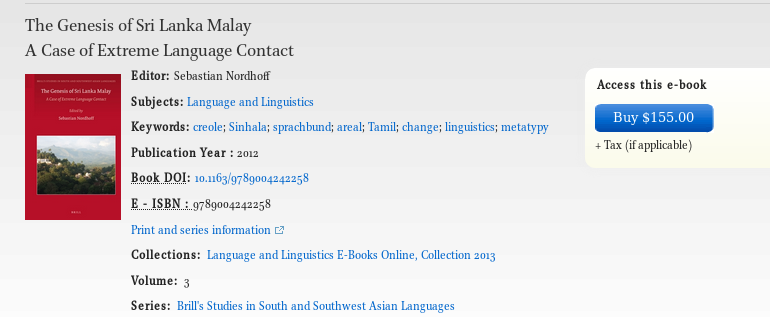
\includegraphics[width=5cm]{brill.png}\hfill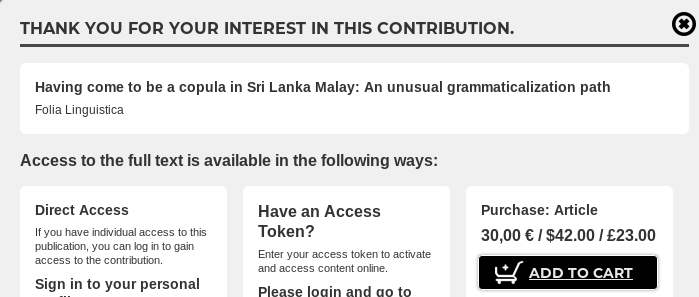
\includegraphics[width=5cm]{folia.png}\\
\vfill
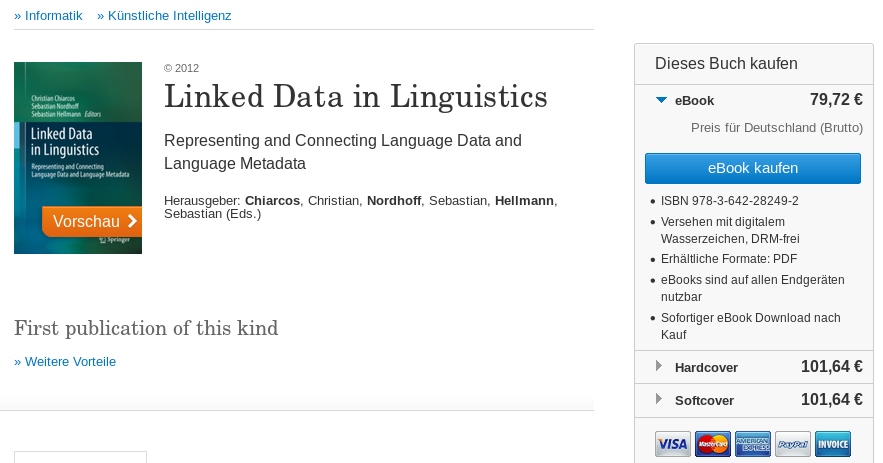
\includegraphics[width=6cm]{springer.png}
\begin{itemize}
 \item als Disziplin sehr OA-freundlich
 \begin{itemize}
  \item Glossa, Language Science Press
 \end{itemize}
\end{itemize}

}

 

\section{Language Science Press}
\frame{
\frametitle{Language Science Press}
%   \includegraphics[height=.2\textheight]{./path/to/graphicsfile}
  \begin{itemize}
    \item linguistische Monographien und Sammelbände als CC-BY
    \item  aktiv seit 2014 (FU Berlin), seit 2017 HU Berlin
    \item  20 Reihen,  160 Herausgeber weltweit 
    \item 45 Bücher, 320 Interessensbekundungen
    \item  930 \textit{public supporters} + 305 ``anonyme Unterstützer''
    \item Plan ab 2018: 30 Bücher pro Jahr
    \item bis zu >20.000 Downloads pro Buch
  \end{itemize}
}

\frame{ 
\frametitle{Was wir publizieren:} 
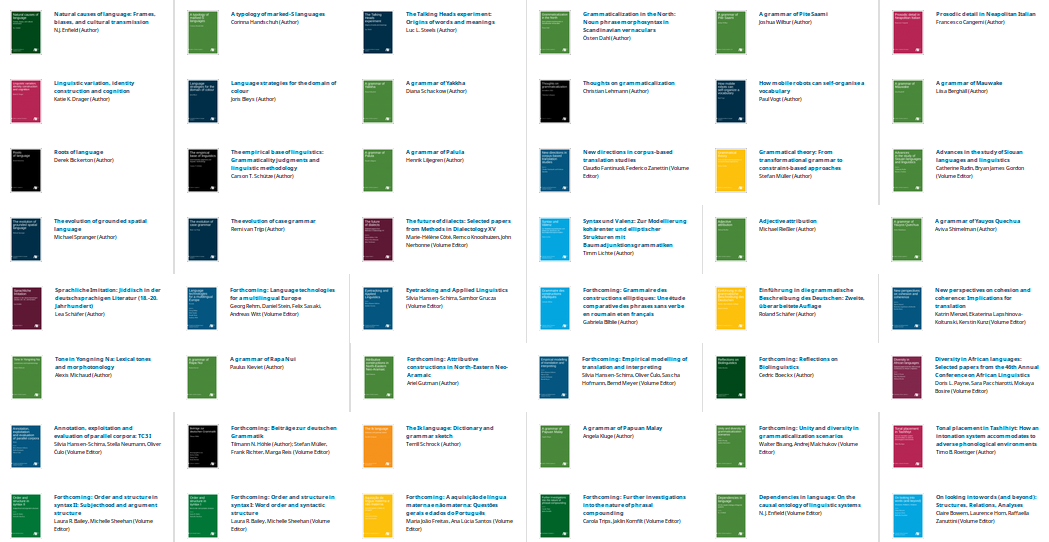
\includegraphics[width=\textwidth]{catalog.png} 
}



\frame{ 
\frametitle{Was wir publizieren:}
\begin{tabular}{ll}
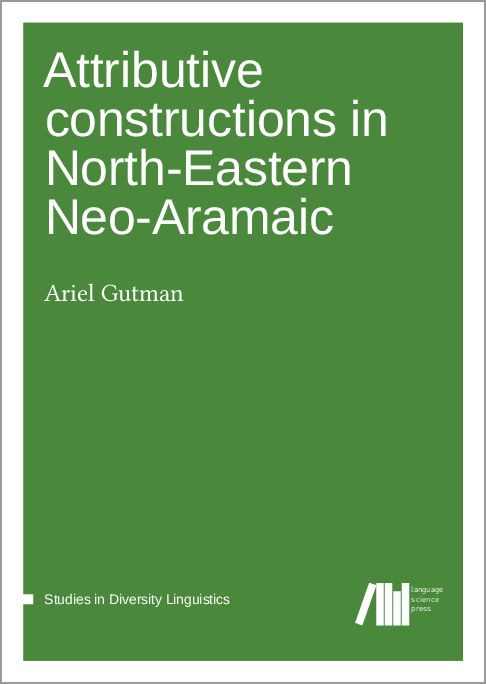
\includegraphics[width=.35\textwidth]{gutman.png}& 
\parbox{.65\textwidth}{
\fbox{
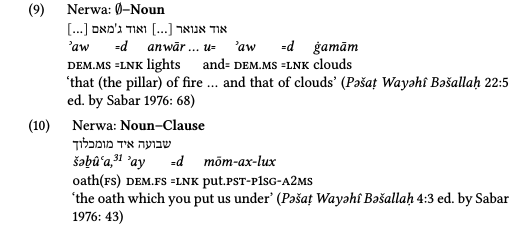
\includegraphics[width=.6\textwidth]{nena.png}  
}
\begin{itemize}
 \item Bücher bis 750 Seiten
 \item teilweise Frucht mehrerer Jahrzehnte Arbeit
 \item Mix zwischen Automatisierung und Maßanfertigung
\end{itemize}

 
\vspace*{6cm}  
}
\end{tabular}
}


% \frame{ 
% \frametitle{Was wir publizieren:}
% \begin{tabular}{ll}
% 
\includegraphics[width=.35\textwidth]{nerbonne.png}& 
% \parbox{.65\textwidth}{
% \fbox{
% 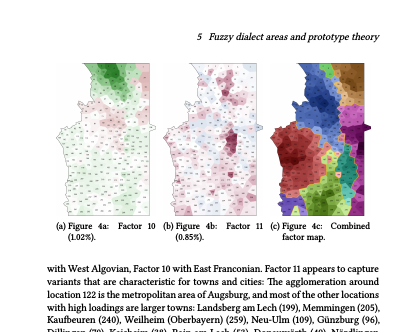
\includegraphics[width=.6\textwidth]{picklmap.png}  
% }
%  
% \vspace*{53mm}  
% }
% \end{tabular}
% }

 


% \frame{ 
% \frametitle{Was wir publizieren:} 
% \begin{tabular}{ll}
% 
\includegraphics[width=.35\textwidth]{mueller.png}& 
% \parbox{.65\textwidth}{
% \fbox{
% 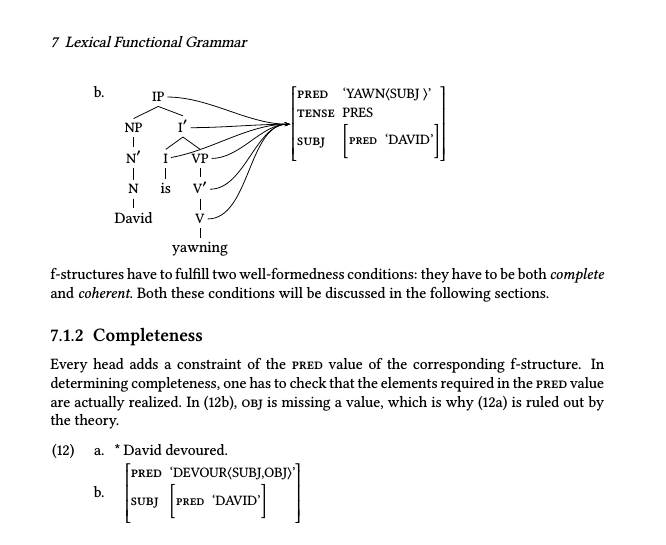
\includegraphics[width=.6\textwidth]{lfg.png}  
% }
%  
% \vspace*{50mm}  
% }
% \end{tabular}
% }


\section{Prinzipien}
% \subsection{Prinzip der Offenheit}

\frame{
\frametitle{Prinzip der Offenheit}
%   \includegraphics[height=.2\textheight]{./path/to/graphicsfile}
  \begin{itemize}
    \item  Nur FLOSS, nur CC-BY, transparente Kalkulationen
  \end{itemize}
  
  
\includegraphics[width=3cm]{omp.png} 
  
\includegraphics[width=3.5cm]{github.png} 
  
\includegraphics[width=4cm]{paperhive.png}
  
  
\includegraphics[width=3cm]{overleaf.png}
  
\includegraphics[width=3cm]{ctan.png}
  
\includegraphics[width=3cm]{oapen.png}
  
\includegraphics[width=3cm]{doab.png}
}
 

% \subsection{Prinzip der Community}
\frame{
\frametitle{Prinzip der Community}
%   \includegraphics[height=.2\textheight]{./path/to/graphicsfile}
  ~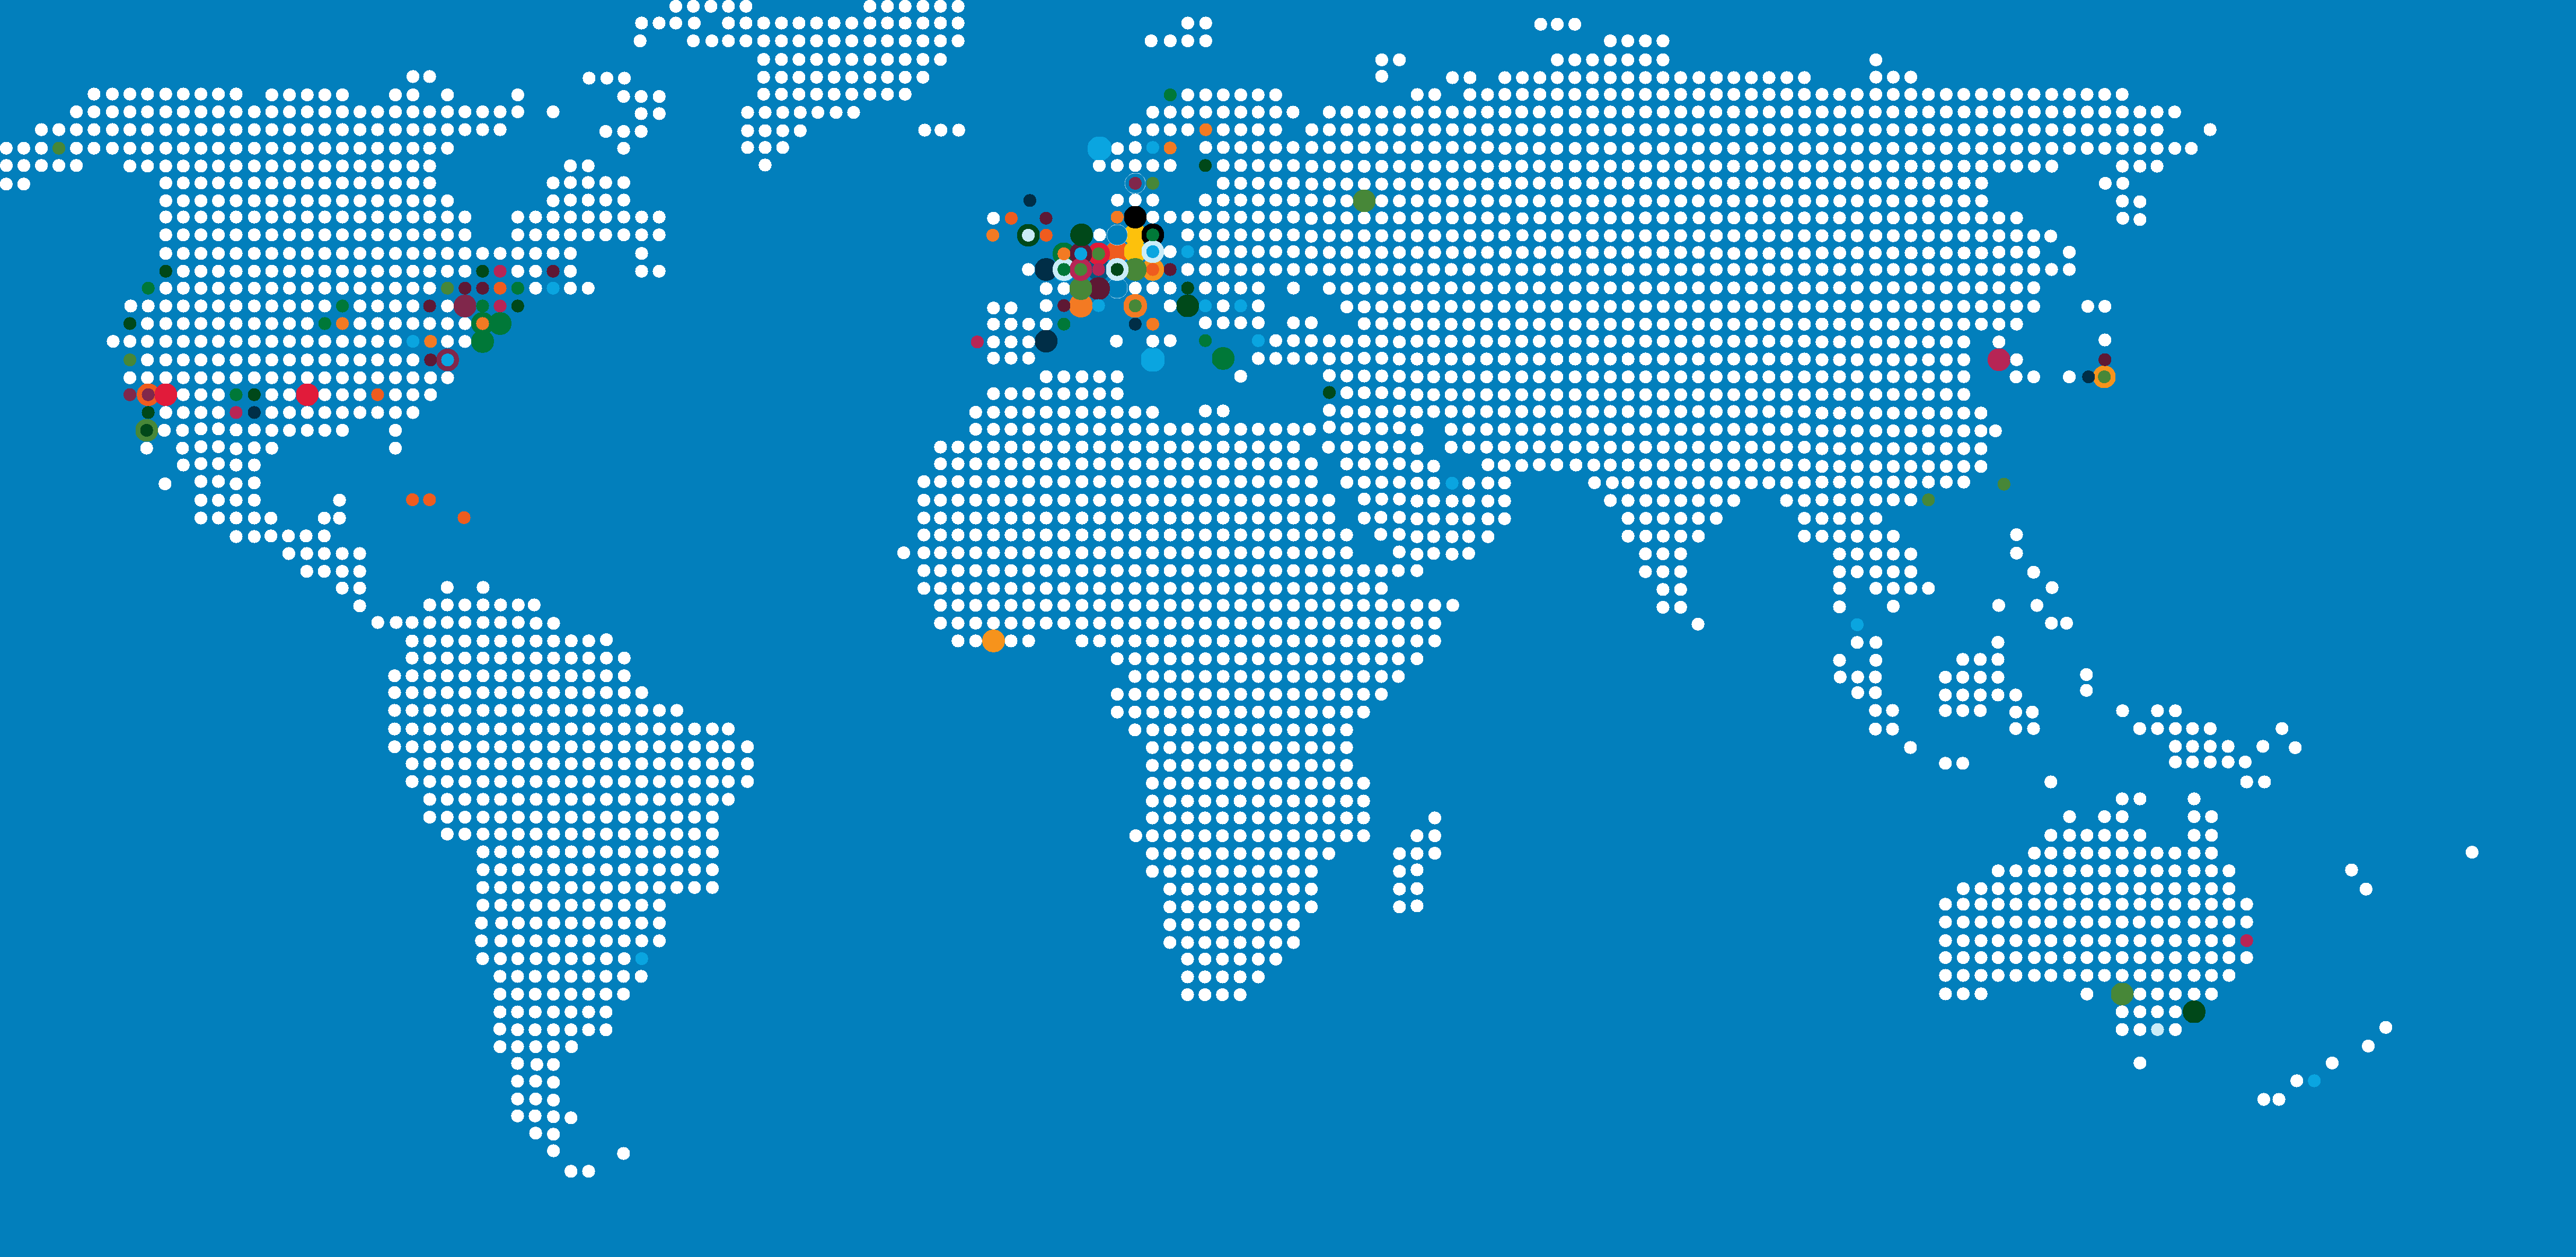
\includegraphics[width=.95\textwidth]{WORLDMAPDOTSdots.png}
  \begin{itemize}
    \item weltweit, autark, dezentral, bottom-up
    \item own the brands (anders als LivingReviews, SSRN,  etc)
    \item share the source
    \begin{itemize}
     \item  Templates, Quelldateien, Geschäftsprozesse, Kalkulationen
    \end{itemize}
  \end{itemize}
}

 
   


% \subsection{Prinzip der Schlankheit}    

\frame{
\frametitle{Prinzip der Schlankheit}
%   \includegraphics[height=.2\textheight]{./path/to/graphicsfile}
  \begin{itemize}
    \item keine Legacy-Software
    \item keine Lagerhaltung
    \item kein Vertrieb
    \item keine IT für Paywalls, Registrierung
    \item kein Marketing 
    \item keine Buchstände
    \item keine komplizierten Autorenverträge 
    \item keine Tantiemen\\$\to$ born digital
  \end{itemize}
}


\section{Workflow}    

\frame{
\frametitle{Workflow}
\begin{columns}
  \begin{column}{5cm} 
\begin{center}
\vspace*{-2mm}
\small
    \fbox{Einreichung}
    
    $\downarrow$
    
    \fbox{(open) peer review \raisebox{-0.5mm}{
\includegraphics[width=3mm]{pdf.jpg}}}
    
    $\downarrow$
    
    \fbox{Überarbeitung}
    
    $\downarrow$
    
    \fbox{Konversion}
    
    $\downarrow$
    
    \fbox{community proofreading \raisebox{-0.5mm}{
\includegraphics[width=3mm]{pdf.jpg}}}
    
    $\downarrow$
    
    \fbox{Satz}
    
    $\downarrow$
    
    \fbox{Veröffentlichung \raisebox{-0.5mm}{
\includegraphics[width=3mm]{pdf.jpg}~
\includegraphics[width=3mm]{doi.png}}}
    
    $\downarrow$
    
    \fbox{Neuauflagen \raisebox{-0.5mm}{
\includegraphics[width=3mm]{pdf.jpg}~
\includegraphics[width=3mm]{doi.png}}}
    
\end{center}
      \end{column}
  \begin{column}{4.2cm}
    \begin{itemize}
      \item Versionen des Dokuments sind als pdf in verschiedenen Stadien verfügbar
      \item Kein Anspruch auf Gatekeeper-Funktion
      \end{itemize}
    \vspace*{2cm}
  \end{column}
\end{columns}
}


\frame{
\frametitle{Voraussetzungen}
%   \includegraphics[height=.2\textheight]{./path/to/graphicsfile}
  \begin{itemize}
  \item Community-Building
  \item keine Gewinnerzielungsabsicht
  \item kein Anspruch auf Verwertungsrechtemonopol
  \item verteilte Finanzierung (konkret: Knowledge Unlatched)
  \item klares inhaltliches Profil
  \item Buchmenge überschaubar und vorhersagbar 
  \item Anerkennungskultur      
  \end{itemize} 
}

\section{Diskussion}

\frame{
\frametitle{Diskussion}
\begin{itemize}
 \item Ist es überhaupt ein Buch? 
 \begin{itemize}
  \item pdf, Quelltext, Grafiken, Rohdaten, Versionshistorie, Makefiles
 \end{itemize}
 \item Ist es überhaupt 1 Buch? 
 \begin{itemize}
  \item Open-Review-Version, Community-Proofreading-Version, Auflage 1, Auflage 2, ...
 \end{itemize}
 \item Probleme von am materiellen Exemplar orientierten Finanzierungsmodellen
 \item Finanzierungsmöglichkeiten
 \begin{itemize}
  \item Library Partnership, Printmarge, {\tiny (Spenden), (individuelle Mitgliedschaften), (Autorengebühren)}
 \end{itemize}

\end{itemize}
}

\frame{
\frametitle{Diskussion}
 \begin{itemize}
  \item starker Wandel im Markt
  \item traditionelles Reader-Pays wird sich nicht mehr lange halten
  \item Big Deals favorisieren Großverlage. 
  \begin{itemize}
   \item Markteintritt wird teuer
  \end{itemize}
  \item ursprüngliche Ziele von Open Access
   \begin{itemize}
    \item besserer Zugang (\checkmark)
    \item billiger (=)
    \item demokratischer (?)
   \end{itemize}
 \end{itemize} 

}
 
\end{document}

